\section{Questions}

\begin{problem}[20]
Determine the equilibrium points of the autonomous system
\begin{align*}
 \dot{x} &= (x-1)(x+y) \\
 \dot{y} &= y-x^2
\end{align*}

Which of these points are stable? Which of them are asymptotically stable? \textbf{Hint:} Obtain the jacobian matrix $A$ at the equilibrium point(s), then apply Lyapunov's indirect method (Theorem 3.7 in Khalil textbook).
\end{problem}

\begin{answer}
	Solving the system by having individual differential equations equal 0, like:
	\begin{align*}
	(x-1)(x+y)=0\\
	y-x^2=0
	\end{align*}
	We obtain (1,1), (0,0), and (-1,1) as equilibrium points. 
	Using Lyapunov's indirect method, we can compute and check whether the Jacobian matrix A is Hurwitz at equilibrium points or not.
	The Jacobian matrix is:
	\begin{align*}
	A = 
 \begin{bmatrix}
	2x+y-1 & x -1 \\
	-2x& 1
	\end{bmatrix}
	\end{align*}
	For (1,1):
	\begin{align*}
	A = 
\begin{bmatrix}
	2 & 0 \\
	-2& 1
	\end{bmatrix}\\
	\lambda_1 = 1\\
	\lambda_2 = 2\\
	\end{align*}
	A is not Hurwitz => Not asymptotically stable at (1,1).
	For (-1,1):
	\begin{align*}
	A =  \begin{bmatrix}
	-2 & 2 \\
	2& 1
	\end{bmatrix}\\
	\lambda_1 = 1\\
	\lambda_2 = -2\\
	\end{align*}
	A is not Hurwitz => Not asymptotically stable at (-1,1).
	For (0,0):
	\begin{align*}
	A =  \begin{bmatrix}
	-1 & -1 \\
	0& 1
	\end{bmatrix} \\
	\lambda_1 = 1\\
	\lambda_2 = -1\\
	\end{align*}
	A is not Hurwitz => Not asymptotically stable at (0,0).
	So system has no asymptotically stable equilibrium points.
\end{answer}

\begin{problem}[20]
Consider the nonlinear system
$$
\begin{array}{l}
\dot{x}_1=-x_1-e^{-2 t} x_2 \\
\dot{x}_2=x_1-x_2
\end{array}.
$$

Determine whether the equilibrium point at 0 is stable or not?
\textbf{Hint:} Use the following Lyapunov function $V(x, t)=x_1^2+\left(1+e^{-2 t}\right) x_2^2$. See Example 3.20 in Khalil textbook.
\end{problem}


\begin{answer}
    Choose $g(t)=e^-2t$
    g(t) is continuously differentiable, and:
    \begin{align*}
    \dot{g}(t) = -2e^-2t \leq e^-2t\\
    0 \leq g(t) \leq k, \forall t \geq 0
    \end{align*}
    Taking $V(t,x) = x_1^2 + [1+g(t)]x_2^2$ as a Lyapunov function candidate, it can be easily seen that
    \begin{align*}
    x_1^2+x_2^2 \leq V(t,x) \leq x_1^2+(1+k)x_2^2, \forall x \in R^2
    \end{align*}
    Hence, V(t) is positive definite, decrescent, and radially unbounded. The derivative is:
    \begin{align*}
    \dot{V}(t,x) = -2x_1^2 + 2x_1x_2-[2+2g(t)-\dot{g}(t)]x_2^2
    \end{align*}
    Using the inequality:
    \begin{align*}
    2+2g(t)-\dot{g}(t) \geq 2 + 2g(t) - g(t) \geq 2
    \end{align*}
    We obtain
    \begin{align*}
    \dot{V}(t,x) \leq -2x_1^2 + 2x_1x_2-2x_2^2 = - [ \begin{bmatrix}
    x_1\\
    x_2
\end{bmatrix}  ^T
 \begin{bmatrix}
    2&-1\\
    -1&2
\end{bmatrix}
\begin{bmatrix}
    x_1\\
    x_2
\end{bmatrix} = -x^TQx
    \end{align*}
\end{answer}

\begin{problem}[40]
    Consider the following Cart-Pole system. Let the state be $q:= [q_1,\,q_2,\,q_3,\,q_4]^\top = [x,\, \dot{x},\, \theta,\, \dot{\theta}]^\top$ and $u$ is the control input that represents the force applied on the cart.

    \begin{align*}
        \dot{q} = f(q,u) = 
        \begin{bmatrix}
            \dot{x} \\
            \frac{u + m \sin{\theta}(l\dot{\theta}^2-g\cos{\theta})}{M+m \sin^2{\theta}} \\
            \dot{\theta} \\
            \frac{u\cos{\theta} + ml\dot{\theta}^2\cos{\theta}\sin{\theta} - (M+m)g \sin{\theta}}{l(M+m\sin^2{\theta})}
        \end{bmatrix}
    \end{align*}

    with $M=3, m = 2, l=1, g=9.8065$.
     
    \begin{center}
        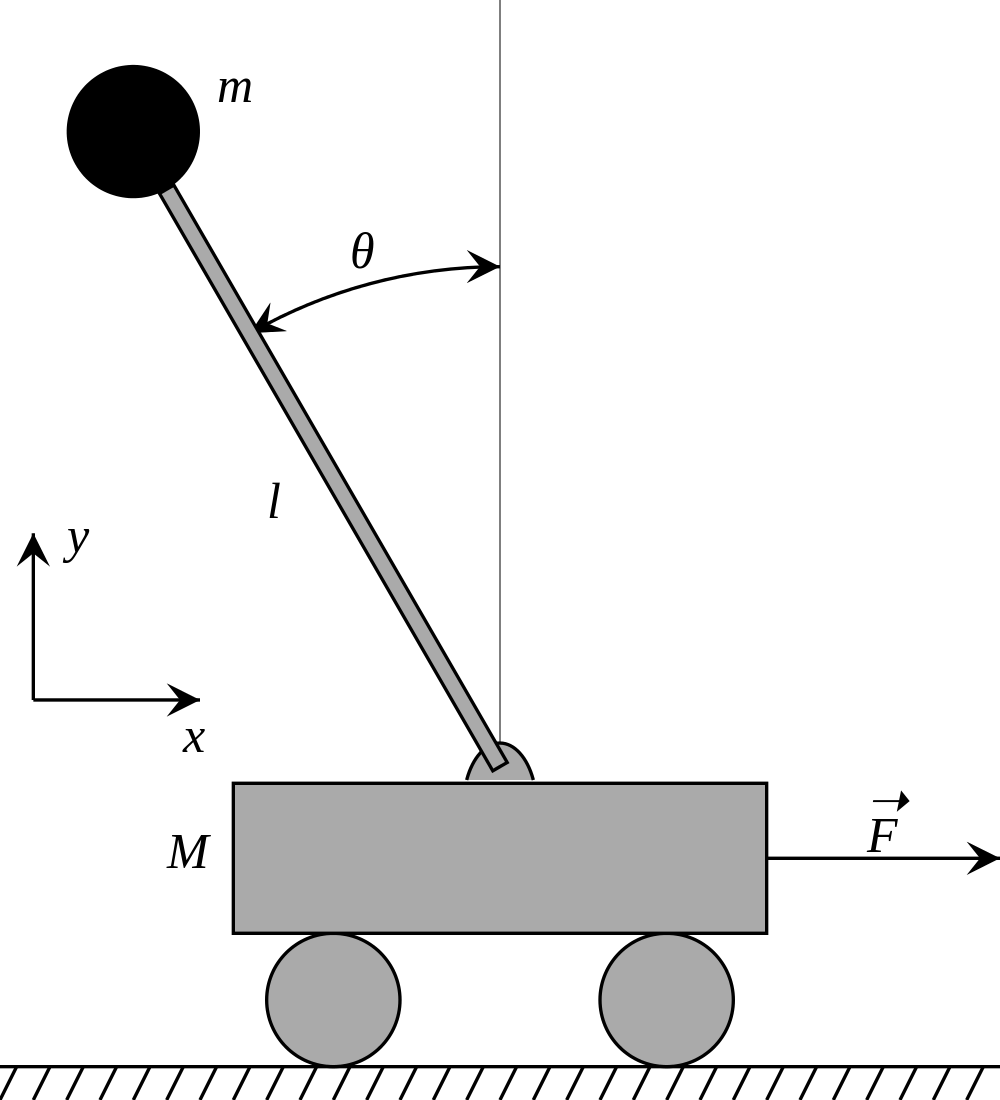
\includegraphics[width=0.3\textwidth]{cart_pole.png}\\
        \tiny{[Image credit: 10.3390/electronics8020198]}
    \end{center}

    Write a script (Python/MATLAB) to answer the following questions:

    \begin{itemize}
        \item Consider zero control input i.e., $u=0$. Notice that $q_e=[0,0,0,0]^T$ is an equilibrium point of the uncontrolled system $\dot{q} = f(q,0)$, corresponding to the upright position of the pole. Is $q_e$ stable or unstable? \textbf{Hint:} Compute $A = \frac{\partial}{\partial q} f(q,0)$ at $q = q_e$ and check if $A$ is a Hurwitz matrix. Directly apply Theorem 3.7 from Khalil textbook.
        \item Now we consider a linear feedback controller $u(q)=-K(q-q_e)$. The point $q_e=[0,0,0,0]^T$ is still an equilibrium point for the closed-loop system $\dot{q} = f(q,u(q))$. For $K=[1,3.371, 1.781, 1.891]$, determine if the equilibrium $q_e$ is now stable or unstable. \textbf{Hint:} Use the same steps as before. Start by computing $A = \frac{\partial}{\partial q} f(q,u(q))$ at $q = q_e$.
        \item Using the $A$ matrix from above, compute a quadratic Lyapunov function of the form $V(q) = q^TPq$ by solving the Lyapunov equation $A^TP+PA=-Q$ with symmetric matrix $Q \succ 0$. You can choose any $Q \succ 0$ you like. \textbf{Hint:} Use can dirtectly use the packages like SciPy or Python Control Systems Library to solve the Lyapunov equation.
        \item Optional bonus question [Extra 10 points]: Set the initial condition for $x$ and $\dot{x}$ to be zero. Through simulations, estimate the region of attraction of $q_e$ in the $\theta-\dot{\theta}$ plane. Plot $\dot{V}(q)$ in the $\theta-\dot{\theta}$ by fixing $x=0,\, \dot{x} = 0.$ Notice that $\dot{V}(q)$ has negative values in some small neighborhood of $q_e.$ \textbf{Hint:} For different values of $q_3,q_4$, start from $(0,0,q_3,q_4)$ and check if system converges to $q_e.$
    \end{itemize}

    NOTE: \textcolor{red}{Please use \href{https://colab.research.google.com/drive/1x2WGCb0C48q0tuzGt1kJMdKYDZ4DN0EO?usp=sharing}{this template} for programming, and if you are unsure how to share online script, please submit the report and script packaged into a compressed '.zip' file.}
    
\end{problem}

\begin{answer}
    YOUR ANSWER HERE.
\end{answer}



